\documentclass[11pt,twocolumn]{article}
\usepackage{graphicx}
\usepackage[left=1.80cm, right=1.80cm, top=2.00cm, bottom=2.00cm]{geometry}
\usepackage{amsmath}
\usepackage[colorlinks]{hyperref}
\usepackage[backend=biber]{biblatex}
\usepackage{eurosym}
\usepackage[dvipsnames]{xcolor}
\usepackage{subcaption}
\usepackage{enumitem} % for alphabetical enumeration 
\usepackage{accents}
\usepackage[capitalise]{cleveref}



\addbibresource{main.bib}
\graphicspath{{../figures/}}

\crefname{relation}{Rel.}{Rels.}
\creflabelformat{relation}{(#2#1#3)}
\crefname{constraint}{Constr.}{Constrs.}
\creflabelformat{constraint}{(#2#1#3)}

\setlength\parindent{8pt}

% style operators
\newcommand{\ie}{\textit{i.e.} }
\newcommand{\eg}{\textit{e.g.} }
\newcommand{\ubar}[1]{\underaccent{\bar}{#1}}
\newcommand{\note}[1]{\textcolor{Orange}{#1}}
\newcommand{\vpad}{\vspace{1mm}}
\newcommand{\hpad}{\hspace{15pt}}
\newcommand{\resultsin}[1]{\hspace{6pt} \bot  \hspace{6pt} #1}
\newcommand{\Forall}[1]{\hspace{10pt} \forall \,\, #1 }
\newcommand{\pdv}[2]{\frac{\partial #1}{\partial #2}}


% general symbols
\newcommand{\generation}{g_{s,t}}
\newcommand{\generationpotential}{\bar{g}_{s,t}}
\newcommand{\generationshare}[1][n]{\omega_{#1,s,t}}
\newcommand{\nodalgeneration}[1][n]{g_{#1,t}}
\newcommand{\capacityGeneration}{G_{s}}
\newcommand{\capacityGenerationUpper}{\bar{G}_{s}}
\newcommand{\capacityGenerationLower}{\ubar{G}_{s}}
\newcommand{\capacityFlow}{F_{\ell}}
\newcommand{\capacityFlowUpper}{\bar{F}_{\ell}}
\newcommand{\capacityFlowLower}{\ubar{F}_{\ell}}
\newcommand{\capexGeneration}{c_{s}}
\newcommand{\capexFlow}{c_{\ell}}
\newcommand{\opexGeneration}{o_{s}}
\newcommand{\demand}[1][n]{d_{#1,t}}
\newcommand{\nodaldemand}[1][n]{d_{#1,t}}
\newcommand{\demandshare}[1][n]{\omega_{#1,a,t}}
\newcommand{\utility}{U_{n,a,t}}
\newcommand{\incidence}[1][n]{K_{#1,\ell}}
\newcommand{\incidenceGenerators}[1][n]{K_{#1,s}}
\newcommand{\ptdf}[1][n]{H_{\ell,#1}}
\newcommand{\ptdfEqual}[1][n]{\ptdf[#1]^\circ}
\newcommand{\slackflow}{k_{\ell}}
\newcommand{\slack}[1][n]{k_{#1}}
\newcommand{\slackk}[1][n]{k^*_{#1}}
\newcommand{\Slack}{k_{m,n}}
\newcommand{\Slackk}{k^*_{m,n}}
\newcommand{\mulowergeneration}{\ubar{\mu}_{s,t}}
\newcommand{\muuppergeneration}{\bar{\mu}_{s,t}}
\newcommand{\mulowerflow}{\ubar{\mu}_{\ell,t}}
\newcommand{\muupperflow}{\bar{\mu}_{\ell,t}}
\newcommand{\lmp}[1][n]{\lambda_{#1,t}}
\newcommand{\flow}{f_{\ell,t}}
\newcommand{\cycle}{C_{\ell,c}}
\newcommand{\impedance}{x_\ell}
\newcommand{\cycleprice}{\lambda_{c,t}}
\newcommand{\injection}{p_{n,t}}
\newcommand{\netconsumption}[1][n]{p^{-}_{#1,t}}
\newcommand{\netproduction}[1][n]{p^{+}_{#1,t}}
\newcommand{\selfconsumption}[1][n]{p^{\circ}_{#1,t}}

\newcommand{\totalnetconsumption}{p^{-}_{t}}
\newcommand{\totalnetproduction}{p^{+}_{t}}
\newcommand{\totalselfconsumption}{p^{\circ}_{t}}
\newcommand{\lagrangian}{\mathcal{L}}

% allocation quantities
\newcommand{\allocatePeer}[1][s \rightarrow n]{A_{#1,t}}
\newcommand{\allocateFlow}[1][n]{A_{\ell,#1,t}}
\newcommand{\allocateTransaction}[1][s \rightarrow n]{A_{#1,\ell,t}}
\newcommand{\allocateCapexGeneration}[1][n]{\mathcal{C}^{G}_{#1,t}}
\newcommand{\allocateCapexFlow}[1][n]{\mathcal{C}^{F}_{#1,t}}
\newcommand{\allocateOpex}[1][n]{\mathcal{O}_{#1,t}}
\newcommand{\allocateEmissionCost}[1][n]{\mathcal{E}_{#1,t}}

\newcommand{\emission}{e_{s}}
\newcommand{\emissionPrice}{\mu_{\text{CO2}}}
\newcommand{\megawatthour}{MWh$_\text{el}$}
\newcommand{\totalcost}{\mathcal{TC}}
\newcommand{\totalOpexGeneration}{\mathcal{O}}
\newcommand{\totalOpexFlow}{\mathcal{O}^F}
\newcommand{\totalCapexGeneration}{\mathcal{C}^G}
\newcommand{\totalCapexFlow}{\mathcal{C}^F}
\newcommand{\totalEmissionCost}{\mathcal{E}}
\newcommand{\totalRest}{\mathcal{R}}



\begin{document}


\title{Flow-Based Cost Allocation in Linear Optimized Power Systems are non-unique but localizable}
\author{F. Hofmann. T. Brown}

\maketitle

\begin{abstract}
Maximizing the welfare of all market participants within a power system is a common approach in energy system modelling. It leads to perfectly scheduled operations of generators and ... 
\end{abstract}




% In the following, we show how Flow Allocation (FA) can be used for decomposing Locational Marginal Prices (LMP) in a linear optimized power system. We begin by revising the fundamentals of the Power Transfer Distribition Factors (PTDF) and the role of the slack, which plays a key role for FA. This will lead us to a generalized form of P2P allocations and transmission usage allocations based on the choice of slack. In a second step, we breakdown the full Lagrangian of a cost-optimization for a network with transmission and generation capacity expansion. By taking into account sensitivities of the flow with respect to changes in the nodal generation, we are able to derive a cost allocation which directly links to FA.  

% \section{Introduction}

\subsubsection*{Nomenclature}

\begin{table}[h]
    \centering
    \begin{tabular}{ll}
        $\lmp$ & Locational Market Price at bus $n$ and  \\ & time step $t$ in \euro/MW \vpad \\
        $\demand$ & Electric demand per bus $n$, demand type $a$, \\ & time step $t$ in MW  \vpad \\
        $\generation$ & Electric generation of generator $s$, \\ & time step $t$  in MW \vpad \\
        $\flow$ & Active power flow on line $\ell$, \\ & time step $t$ in MW   \vpad \\
        $\opexGeneration$ & Operational price in \euro/MW \vpad \\
        $\capexGeneration$ & Capital Price in \euro/MW \vpad \\
        $\capexFlow$  & Capital Price in \euro/MW for transmission \\ & capacity on line $\ell$  \vpad \\
        $\capacityGeneration$ & Generation capacity in MW \vpad \\
        $\capacityFlow$ & Transmission capacity in MW \vpad \\
        $\incidence$ & Incidence matrix \vpad 
    \end{tabular}
\end{table}

\section{Economic Context}

In long-term operation and investment planning models, the total costs $\totalcost$ of a power system include all operational expenditures (OPEX) $\totalOpexGeneration$ and capital expenditures (CAPEX) $\totalCapexGeneration$ and $\totalCapexFlow$ for production  and transmission respectively, thus
\begin{align}
\totalcost &= \totalOpexGeneration + \totalEmissionCost +  \totalCapexGeneration +  \totalCapexFlow + ...
\label{eq:total_cost_terms}
\end{align}
In a network design with minimal $\totalcost$, the Locational Market Price (LMP) describes the marginal price for an incremental increase of electricity demand $\demand$ of any consumer $a$ at bus $n$. It is given by the derivative of the total system cost $\totalcost$ with respect to the local demand $\demand$
\begin{align}
\lmp = \pdv{\,\totalcost}{\,\demand}
\label{eq:total_cost_derivative}
\end{align}
% 
\begin{figure}[h]
\centering
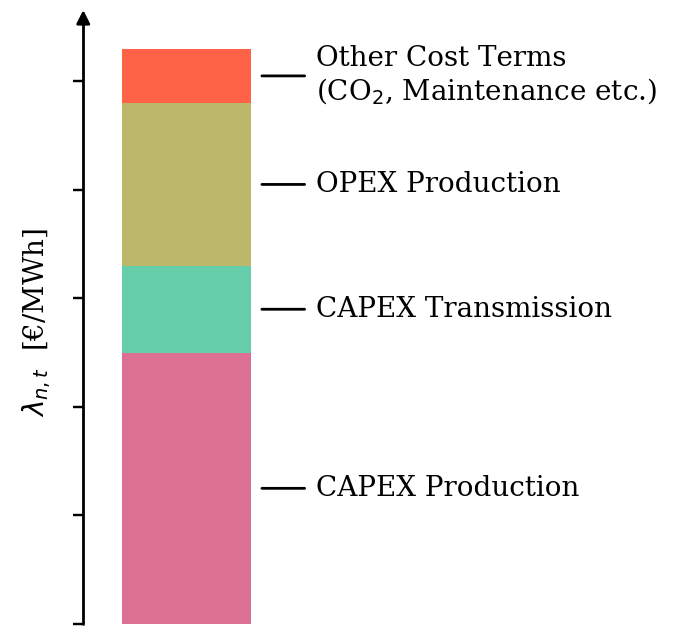
\includegraphics[width=.8\linewidth]{price_decomposition.png}
\caption{Schematic decomposition of the Locational Market Price $\lmp$. In power system model with optimal long-term operation and planning, the total system costs $\totalcost$ split into different cost terms, \ie OPEX and CAPEX for production and transmission and possibly other expenditures. }
\label{fig:price_decomposition}
\end{figure}
% 

This leads to a nodal pricing where over the span of optimized timesteps $t$, the system costs are partially or totally payed back by the consumers 
\begin{align}
\totalcost - \totalRest &=  \sum_{n,a,t} \lmp \, \demand
\label{eq:total_cost_sum}
\end{align}
depending on the costs $\totalRest$ which are independent of the nodal demand  
\begin{align}
 \pdv{\totalRest}{\demand} = 0
\end{align}
% 
In most cases, where $\totalRest$ plays a minor role, the LMP splits into different cost terms assigned to OPEX and CAPEX for production and transmission and eventual other expenditures. We schematically show this behaviour in \cref{fig:price_decomposition}. 
Extensive investigations of the LMP as done in \cite{schweppe_spot_1988} already showed this connection however leave the question open how the costs are allocated among the components. In the following we will show how the above presented cost decomposition is extended to full peer-to-peer (P2P) cost allocation including all network components. 



\section{Nodal Cost Allocation}
\label{sec:theory}

From inserting \cref{eq:total_cost_terms} into \cref{eq:total_cost_derivative}, we are able to disaggregate the cost terms $\totalOpexGeneration$, $\totalCapexGeneration$ and $\totalCapexFlow$ into constributions of demand $\demand$ at bus~$n$ and time~$t$. For the CAPEX allocation we will make use of the shadowprices resulting from the cost mimization. 


\subsection{Allocate Operation Expenditures}

The total OPEX is given by the operational price $\opexGeneration$ times the generation $\generation$ of all generators $s$, 
\begin{align}
 \totalOpexGeneration& = \sum_{s,t} \opexGeneration\,  \generation 
\label{eq:opex_generation}
 \end{align}
The allocated OPEX $\allocateOpex$ which naturally sum up to $  \totalOpexGeneration = \sum_{n,t} \allocateOpex$, are given by 
\begin{align}
\allocateOpex  = \pdv{\totalOpexGeneration}{\demand} \, \demand & =  \sum_{s,t}\opexGeneration \, \pdv{\generation}{\demand} \, \demand
\end{align}
% 
The derivative on the right hand side time the nodal demand can be interpreted as power produced by generator $s$ and consumed at node $n$. Without further explaining how the derivative is calculated, we define this power allocation as 
\begin{align}
 \allocatePeer = \pdv{\generation}{\demand} \, \demand
 \label{eq:allocate_peer}
\end{align}
% 
which by feeding back into \cref{eq:opex_generation} has to fulfill
\begin{align}
\generation = \sum_n \allocatePeer
\label{eq:allocate_peer_constraint}
\end{align}
% 
% 
The direct payment of node $n$ to generator $s$ is then given by  
% 
\begin{align}
 \allocateOpex[n \rightarrow s] &= 
\opexGeneration \,  \allocatePeer
\label{eq:allocate_opexGeneration_detailed}
\end{align}
Accordingly, consumers at bus $n$ which retrieve power from a generators $s$, directly  compensate its operational costs. The cost allocation behaves like P2P tradings between producers and consumers for fixed production prices. In this way, the generator $s$ retrieves the exact amount of money from consumers that it spends on its operation, thus 
\begin{align}
\sum_{n} \allocateOpex[n \rightarrow s] = \opexGeneration \, \generation
\label{eq:no_profit_opex}
\end{align}

\subsection{Allocate Emission Expenditures}

Given a fix price for emissions in CO$_2$ equivalents $\emissionPrice$, the cost term for emission adds up to 
\begin{align}
 \totalEmissionCost = \emissionPrice \, \sum_s  \emission \, \generation
\end{align}
where $\emission$ denotes the emission factor in tonne-CO$_2$ per \megawatthour for generator $s$.
Similar to the allocated OPEX, the emission cost for consumers at bus $n$ at time $t$ is allocated through
\begin{align}
 \allocateEmissionCost = \pdv{\totalEmissionCost}{\demand} \demand = \sum_s \emissionPrice \, \emission \, \allocatePeer  
\end{align}
with its peer-to-peer payments 
\begin{align}
 \allocateEmissionCost[n \rightarrow s] = \emissionPrice \, \emission \, \allocatePeer
\end{align}


\subsection{Allocate Capital Expenditures for Generators}

The optimization of the generation capacity $\capacityGeneration$ adds the cost term 
\begin{align}
 \totalCapexGeneration& = \sum_{s} \capexGeneration \capacityGeneration 
\end{align}
to $\totalcost$. It combines all capacities times their capital cost $\capexGeneration$. The nominal capacity constraints the generation $\generation$ in the form of 
\begin{align}
\generation - \generationpotential \capacityGeneration  &\le 0 \resultsin{\muuppergeneration} \Forall{n,s,t} 
\label[constraint]{eq:upper_generation_capacity_constraint}\\ 
- \generation &\le 0 \resultsin{\mulowergeneration} \Forall{n,s,t} 
\label[constraint]{eq:lower_generation_capacity_constraint}
\end{align}
where $\generationpotential \in \left[ 0,1\right]$ is the capacity factor for renewable generators. Using the result of \cite{brown_decreasing_2020} we show in that the capital cost  for generator $s$ translates is payed back by the generation times the shadow price for the upper capacity constraint, 
\begin{align}
 \capexGeneration \capacityGeneration = \sum_t \muuppergeneration \,  \generation 
 \label{eq:no_profit_capex_generation}
\end{align}
With our definition in \cref{eq:allocate_peer} the allocated CAPEX can then be defined as 
\begin{align}
\allocateCapexGeneration = \pdv{\totalCapexGeneration}{\demand} \, \demand & = \sum_{s} \muuppergeneration \, \allocatePeer
\end{align}
with the peer-to-peer allocation 
\begin{align}
 \allocateCapexGeneration[n \rightarrow s] = \muuppergeneration \, \allocatePeer
 \label{eq:allocate_capexGeneration_detailed}
\end{align}

So, how does this allocation behave? According to the polluter pays principle, it differentiates between consumers who are `responsible` for investments and those who are not. If $\muuppergeneration$ (in literature often denoted as the Quality of Supply) is bigger than zero, the upper Capacity \cref{eq:upper_generation_capacity_constraint} is binding. Thus it is these times steps which push investments in $\capacityGeneration$. If $\muuppergeneration = 0$, the generation $\generation$ is not bound and investments are not necessary. 
When summing over all CAPEX payments to generator $s$ in \cref{eq:allocate_capexGeneration_detailed} and using \cref{eq:allocate_peer_constraint,eq:no_profit_capex_generation}, we see that each generator retrieves exactly the cost that were spent to build the capacity $\capacityGeneration$.
 

\subsection{Allocate Capital Expenditures for Transmission Lines}


The CAPEX for the transmission system is given by 
\begin{align}
 \totalCapexFlow & = \sum_\ell \capexFlow \capacityFlow
 \label{eq:capex_flow}
\end{align}
The transmission capacity variable $\capacityFlow$ limits the flow $\flow$ in both directions, such that 
\begin{align}
\flow - \capacityFlow &\le 0 \resultsin{\muupperflow} \Forall{\ell,t} 
\label[constraint]{eq:upper_flow_capacity_constraint} \\
- \flow - \capacityFlow &\le 0 \resultsin{\mulowerflow} \Forall{\ell,t} 
\label[constraint]{eq:lower_flow_capacity_constraint}
\end{align}
Again, we use the result of \cite{brown_decreasing_2020} which derives that the investment in line $\ell$ is payed back by the shadowprices times the flow 
\begin{align}
\capexFlow \capacityFlow = \sum_{t} \left( \muupperflow - \mulowerflow \right)  \flow 
\label{eq:no_profit_capex_flow}
\end{align}
We insert this into \cref{eq:capex_flow} and define the individual cost terms  as 
\begin{align}
\allocateCapexFlow = \pdv{\totalCapexFlow}{\demand}\demand & =  \sum_{\ell,t} \left( \muupperflow - \mulowerflow \right) \pdv{\flow}{\demand} \, \demand
\end{align}
The marginal change of flow with repect to the nodal demand is again non-unique and requires assumption on where the power is resulting from. 

\begin{align}
 \pdv{\flow}{\demand}\, \demand = \allocateFlow
\end{align}
fulfilling 
\begin{align}
\sum_{n} \allocateFlow = \flow 
\label{eq:allocate_transaction_constraint}
\end{align}
% 
The peer-to-peer cost allocation for the transmission CAPEX is then defined as 
\begin{align}
 \allocateCapexFlow[n \rightarrow \ell] &=  
\left( \muupperflow - \mulowerflow\right)  \allocateFlow
\label{eq:allocate_capexFlow_detailed}
\end{align}
% 
Again we can interpret the shadowprices $\muupperflow$ and $\mulowerflow$ as a measure for necessity of transmission investments at $\ell$ at time $t$. Consumers which retrieve power flowing on congested lines, yielding a bound \cref{eq:upper_flow_capacity_constraint} or \eqref{eq:lower_flow_capacity_constraint}, pay compensations for the resulting investments. Again the sum of all CAPEX payments to line $\ell$ equals the total CAPEX spent. This is seen when summing \cref{eq:allocate_capexFlow_detailed} over all buses and time steps and using \cref{eq:allocate_transaction_constraint,eq:no_profit_capex_flow}
 

% \subsection{LMP independent Cost  Terms}
% 
% Example: \\
% Constraining the capacities $\capacityGeneration$  for a subset $S$ of generators to lower or upper limits in the form of 
% \begin{align}
% \capacityGeneration \ge \capacityGenerationLower \hpad \forall{n,s \in S} \\
% \capacityGeneration \le \capacityGenerationUpper \hpad \forall{n,s \in S}
% \end{align}
% or doing likewise with a subset $L$ of transmission lines,
% \begin{align}
% \capacityFlow \ge \capacityFlowLower \hpad \forall{\ell \in \textit{L}} \\
% \capacityFlow \le \capacityFlowUpper \hpad \forall{\ell \in \textit{L}}
% \end{align}
% does not have any effect on the above presented allocation in \cref{eq:lmp_allocation}. The additional cost directly translate to the Quality of Supply $\muuppergeneration$ for production and $\muupperflow - \mulowerflow$ for transmission respectively. This also counts for limiting the overall production capacity $\sum_{n,s}\capacityGeneration$ or transmission capacity $\sum_\ell \capacityFlow$. However it will distort the no profit rule for generators \cref{eq:no_profit_capex_generation} and transmission \cref{eq:no_profit_capex_flow} respectively. As shown in \cite{brown_decreasing_2020}


\section{Assumptions on Power Allocations}
% \section{\texorpdfstring{Extended Solution Space of $\boldsymbol{\slackk[m]}$}{Solution Space of the Slack}}
\label{sec:localizing_allocations}

The P2P cost allocation suits for any type of topology and network setup. But so far, the question of how $\allocatePeer$ and $\allocateFlow$ are defined was left open. We recap that both rely on derivatives of $\generation$ and $\flow$  with respect to the nodal demand $\demand$ fulfilling \cref{eq:allocate_peer_constraint,eq:allocate_transaction_constraint}. \\
% 
In a first step we will show how the power flow allocation $\allocateFlow$ is linked to the peer-to-peer allacations $\allocatePeer$. Let $\ptdf$ denote Power Transfer Distribition Factors (PTDF) giving the changes in the flow on line $\ell$ for one unit (typically one MW) of net power production at bus $n$.  Further let $\incidenceGenerators$ be 1 if generator $s$ is attached to bus $n$ and zero otherwise. We start from the linear power flow equation
\begin{align}
 \flow  = \sum_m \ptdf[m] \left( \nodalgeneration[m] - \demand[m] \right)  
\end{align}
where the nodal generation $\nodalgeneration[m] = \sum_s \incidenceGenerators[m] \, \generation $ combines the production of all generators attached to bus $m$. Taking the derivative with respect to the demand, leads to 
\begin{align}
 \allocateFlow = \pdv{\flow}{\demand} \demand = \sum_m \ptdf[m] \left( \allocatePeer[m \rightarrow n]  - \delta_{n,m} \demand \right) 
 \label{eq:allocate_peer_to_allocate_flow}
\end{align}
where $\allocatePeer[m \rightarrow n] = \sum_s \incidenceGenerators \, \allocatePeer$ combines all power allocations of the source $m$. \Cref{eq:allocate_peer_to_allocate_flow} shows that the peer-to-peer allocation $\allocatePeer$ directly determines the flow allocation on line $\ell$.

 
This leaves us with only solving \cref{eq:allocate_peer_constraint} for $\allocatePeer$. In fact, we have to answer the question of how much power supply does generator $s$ deliver to bus $n$. Unfortunately, the solution is non-unique and requires further assumptions. Established flow allocation schemes approach this problem from different directions. Principally two options exist \textit{what} is allocated 
% 
\begin{enumerate}
\item gross power injections \label{gross}
\item net power injections \label{net}
\end{enumerate}
% 
Further it is important \textit{what assumptions} define the allocation, \ie what method is used to define the pairs of sources and sinks. The three suitable approaches we present here are
% 
\begin{enumerate}[label=\alph*., ref=\alph*]
\item Equivalent Bilateral Exchanges (EBE) \cite{galiana_transmission_2003} which assumes
that every producer supplies every consumer proportional to its share in the total consumption. \label{ebe} 
\item Average Participation (AP) \cite{bialek_tracing_1996,achayuthakan_electricity_2010-1} which traces the flow from producer to consumer following the law of proportional sharing. \label{ap}
\item Flow Based Market Coupling (FBMC) which uses zonal PTDF for allocating power within predefined regions. The interregional exchange is only allocating net power decifit or excess of the regions. \label{fbmc}
\end{enumerate}
% 
We show the mathematical formulation for all combinations \ref{ebe}\ref{gross} - \ref{fbmc}\ref{net} in \cref{sec:gross_ebe,sec:net_ebe,sec:gross_ap,sec:net_ap}.
% 
Principally, type \ref{net} leads to less P2P trades then type \ref{gross} as power from a bus $n$ with $\nodalgeneration \le \nodaldemand$ is not assigned to other buses, only to $n$. 
Further, as literature has often pointed out, the EBE principal \ref{ebe} does not suit for large networks where remote buses would interconnect in the same way as buses in close vicinity \cite{gil_multiarea_2005}. The AP based type \ref{ap} tackles this problem by restricting P2P trades to those which are traceable when applying the proportional sharing principal. Therefore $\allocatePeer$ denotes that part of power produced by bus $m$ which, when only following in the direction of $\flow$, ends up at bus $n$. Type \ref{fbmc} further allows to control the regions or market zones which are netted out in a first calculation. If in a region $R$ the generation undercuts the demand, $\sum_{n \in R} \generation \le \sum_{n \in R} \demand$, none of the inner-regional generation is assigned to other regions. 



\subsection{Numerical Example}
\label{sec:numerical_example}


In the following we showcase a two bus system with one optimized time step and its resulting allocated payments, illustrated in \cref{fig:example_network}. \\
% 
% 
\begin{figure*}[t]
\centering
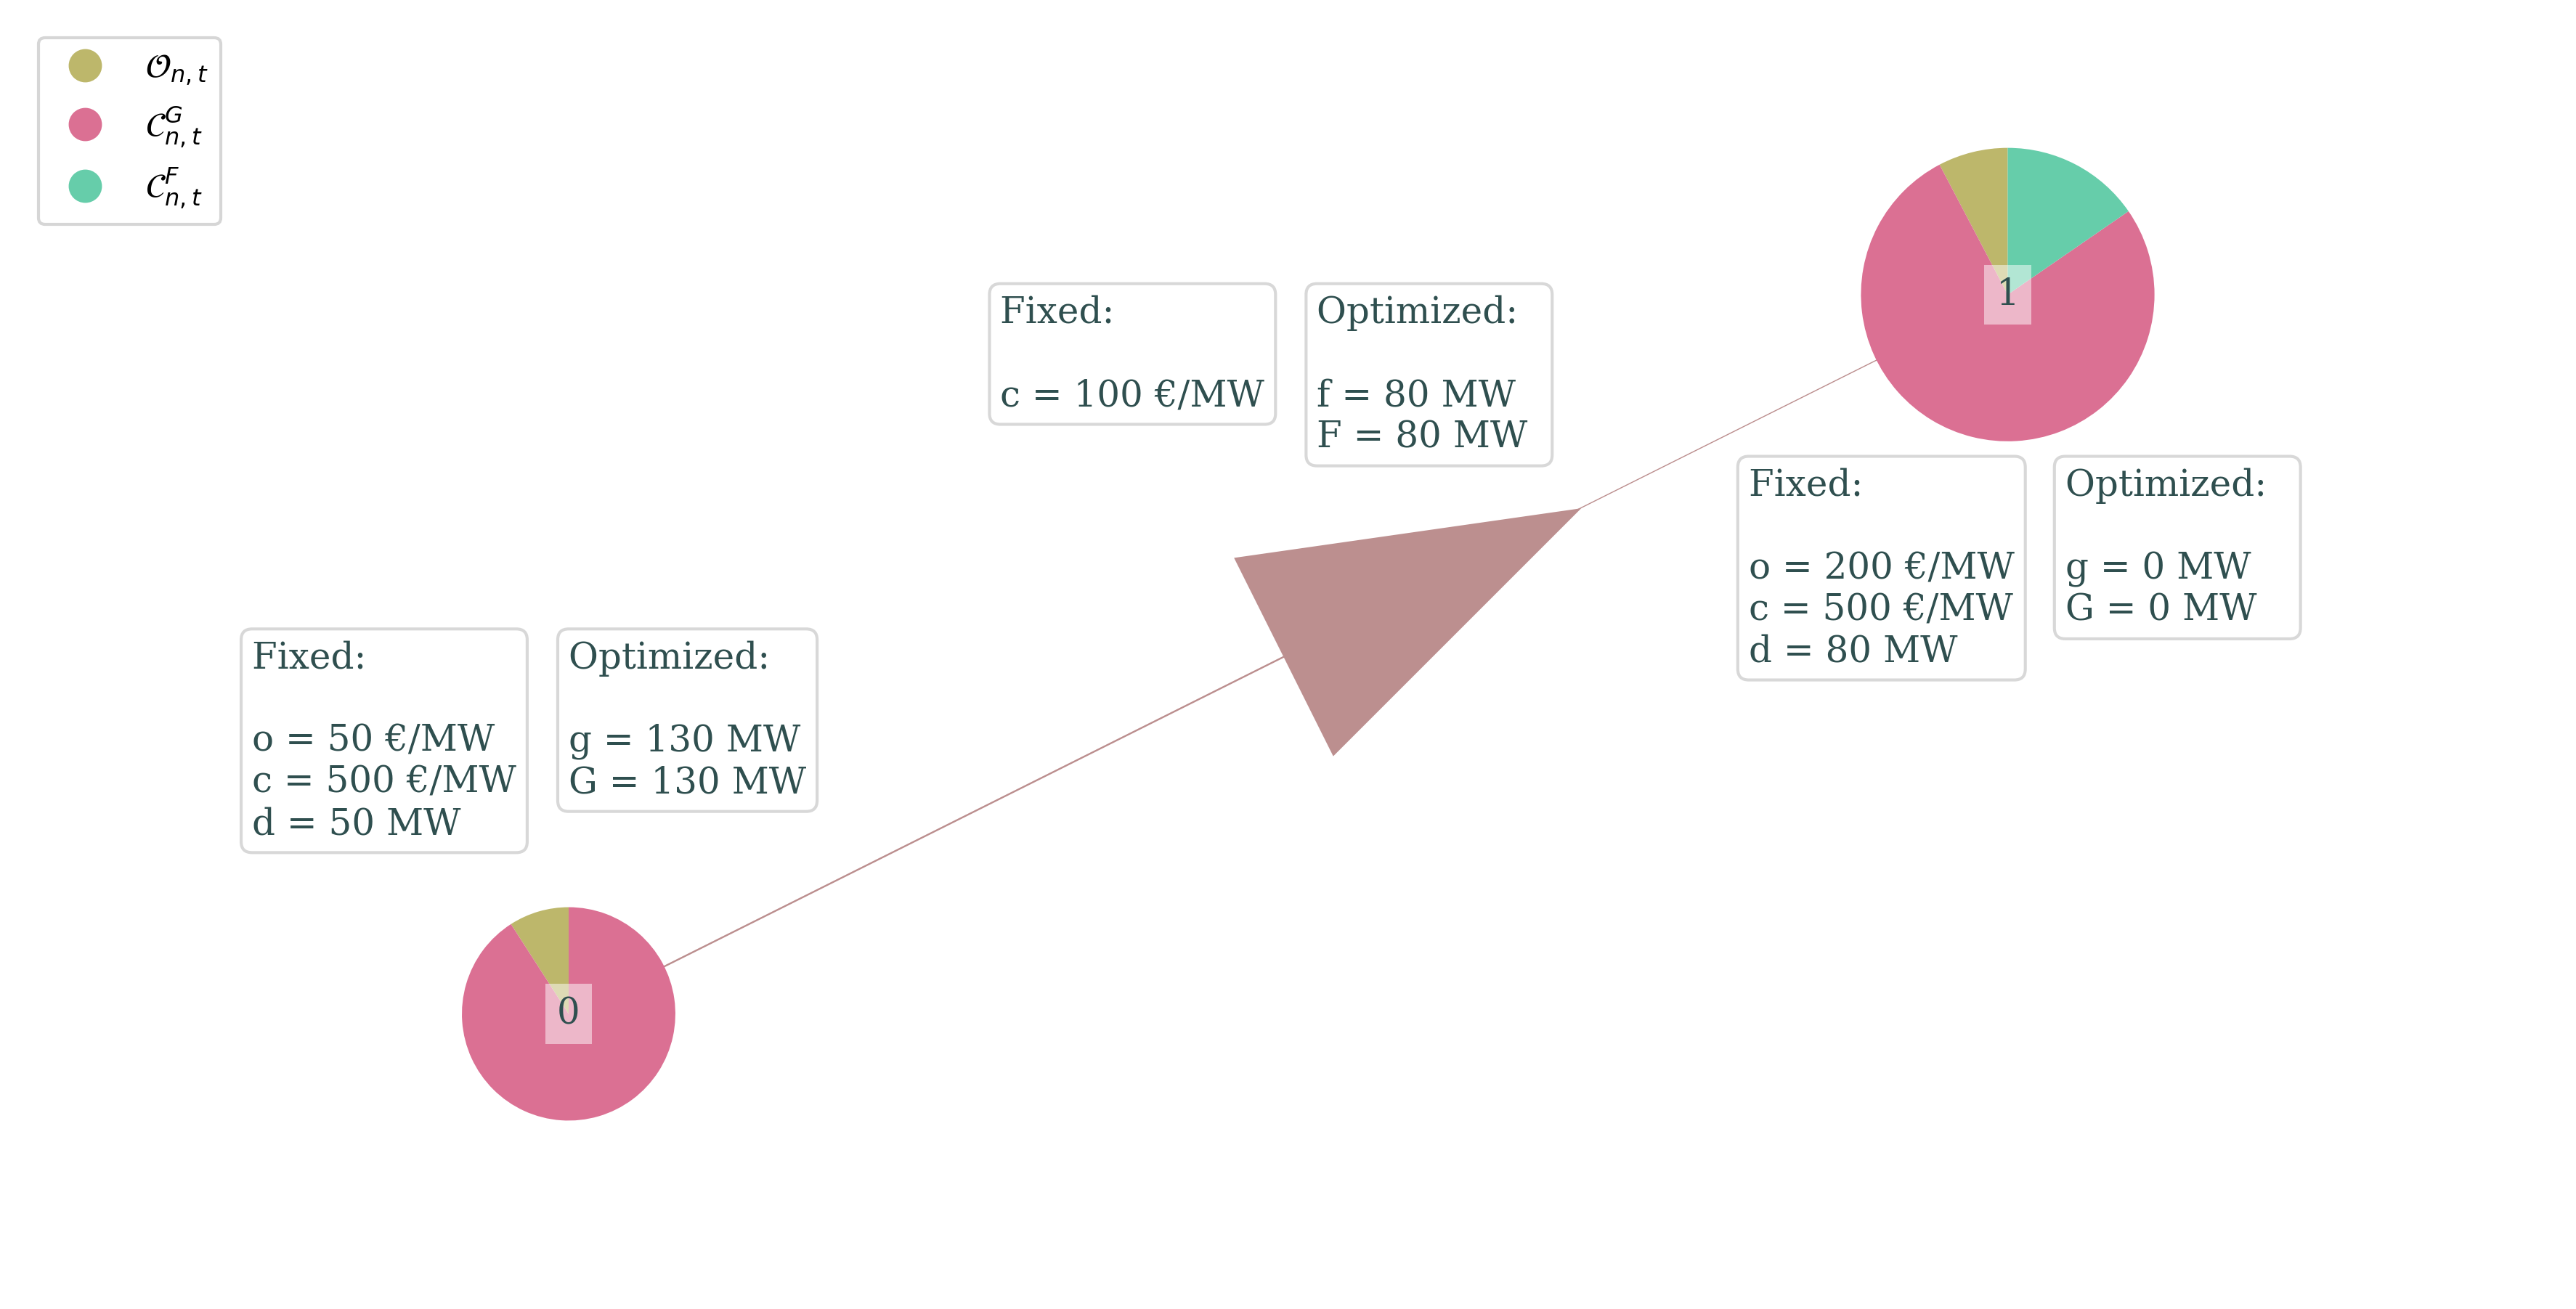
\includegraphics[width=\linewidth]{example_network.png}
\caption{Illustrative example of a 2-bus network with one optimized time step. Fixed prices and constraining values are given in the left box for each bus and the transmission line. Optimized values are given in the right boxes. Bus~1 has a cheaper operational price $o$, capital prices are the same for both. As both generator capacities are constraint to 100~MW, the optimization also deploys the generator at bus~2. The resulting electricity prices $\lambda$ are then a composition of all prices for operation and capital investments. \vspace{-10pt}}
\label{fig:example_network}
\end{figure*}
% 
% 
The two buses are connected via one transmission line, each has one generator. Whereas the generator at bus~1 has an operational price of 50 \euro/\megawatthour, the generator at bus~2 has a higher operational price of 200~\euro/\megawatthour. For both the CAPEX rate is set to 500~\euro/MW and the maxmimal capacity is limited to $\capacityGenerationUpper$~=~100~MW. The transmission line has a CAPEX rate of 100~\euro/MW and no upper capacity limit. With a demand of 60~MW at bus~1 and 90~MW at bus~2, the optimization expands the cheaper generator at bus~1 to its full limit of 100~MW. The 40~MW excess power not consumed at bus~1, flow to bus~2 where the generator is built with only 50~MW.  \\
% 
% 
\begin{figure}[h!]
    \begin{subfigure}[c]{\linewidth}
    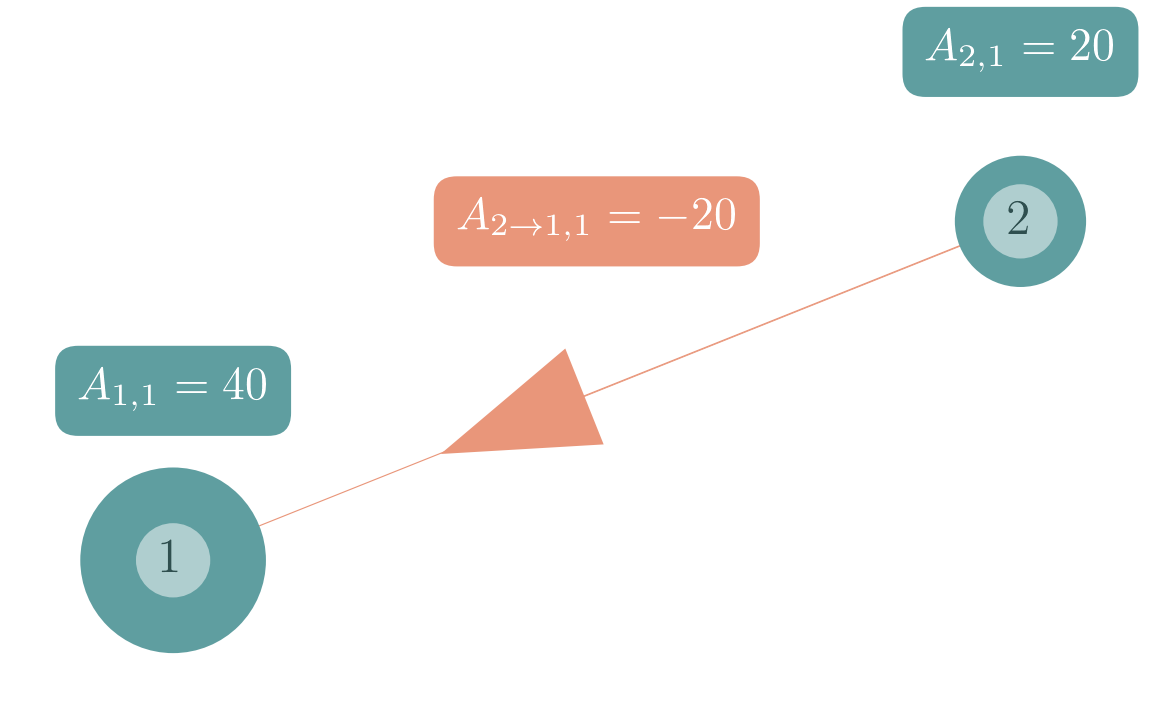
\includegraphics[width=\linewidth]{example_allocation_bus1.png}
    \vspace{-40pt}
    \subcaption{}
    \label{fig:example_allocation_bus1}
    \end{subfigure}
    \begin{subfigure}[c]{\linewidth}
    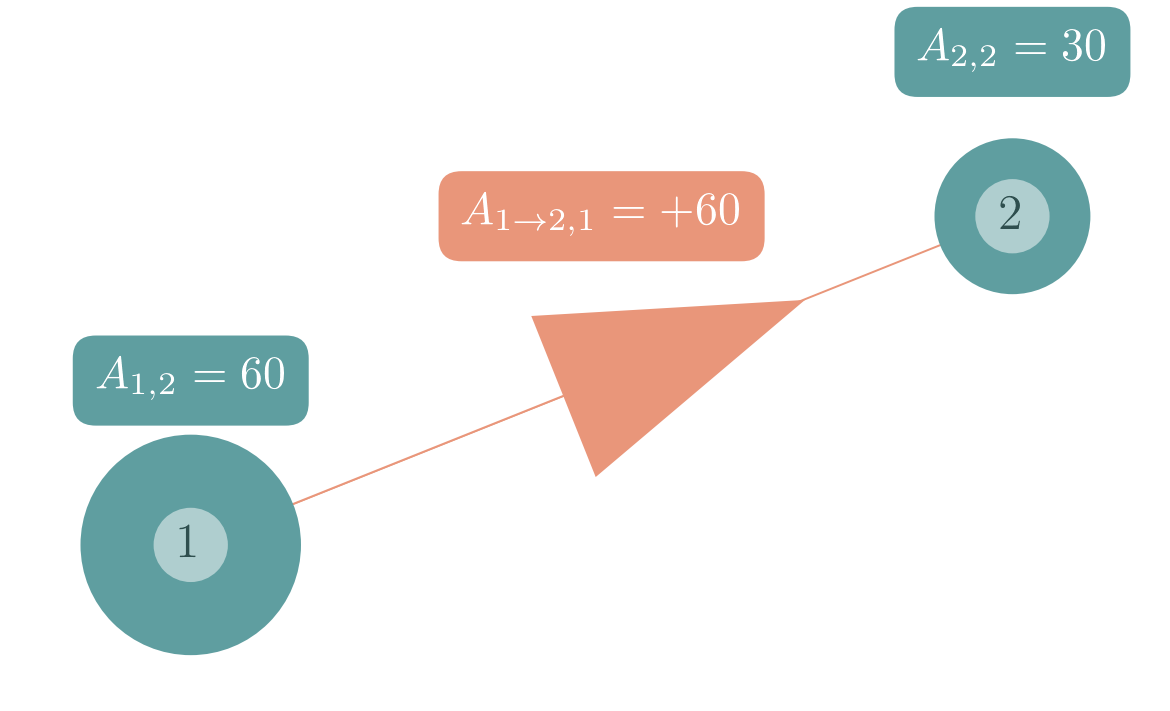
\includegraphics[width=\linewidth]{example_allocation_bus2.png}
    \vspace{-40pt}
    \subcaption{}
    \label{fig:example_allocation_bus2}
    \end{subfigure}
    \caption{Power allocations for bus~1 (a) and bus~2 (b) of the example network in \cref{fig:example_network}. Bus~1 retrieves 40~MW from itself and 20~MW from bus~2. The latter in turn retrieves 60~MW from bus~1 and self supplies 30~MW.
    The sum of both net flows equals the resulting flow of $f=40$~MW. \vspace{-20pt}}
    \label{fig:example_allocation}
\end{figure}
% 
% 
% 
\begin{figure}[h]
\centering
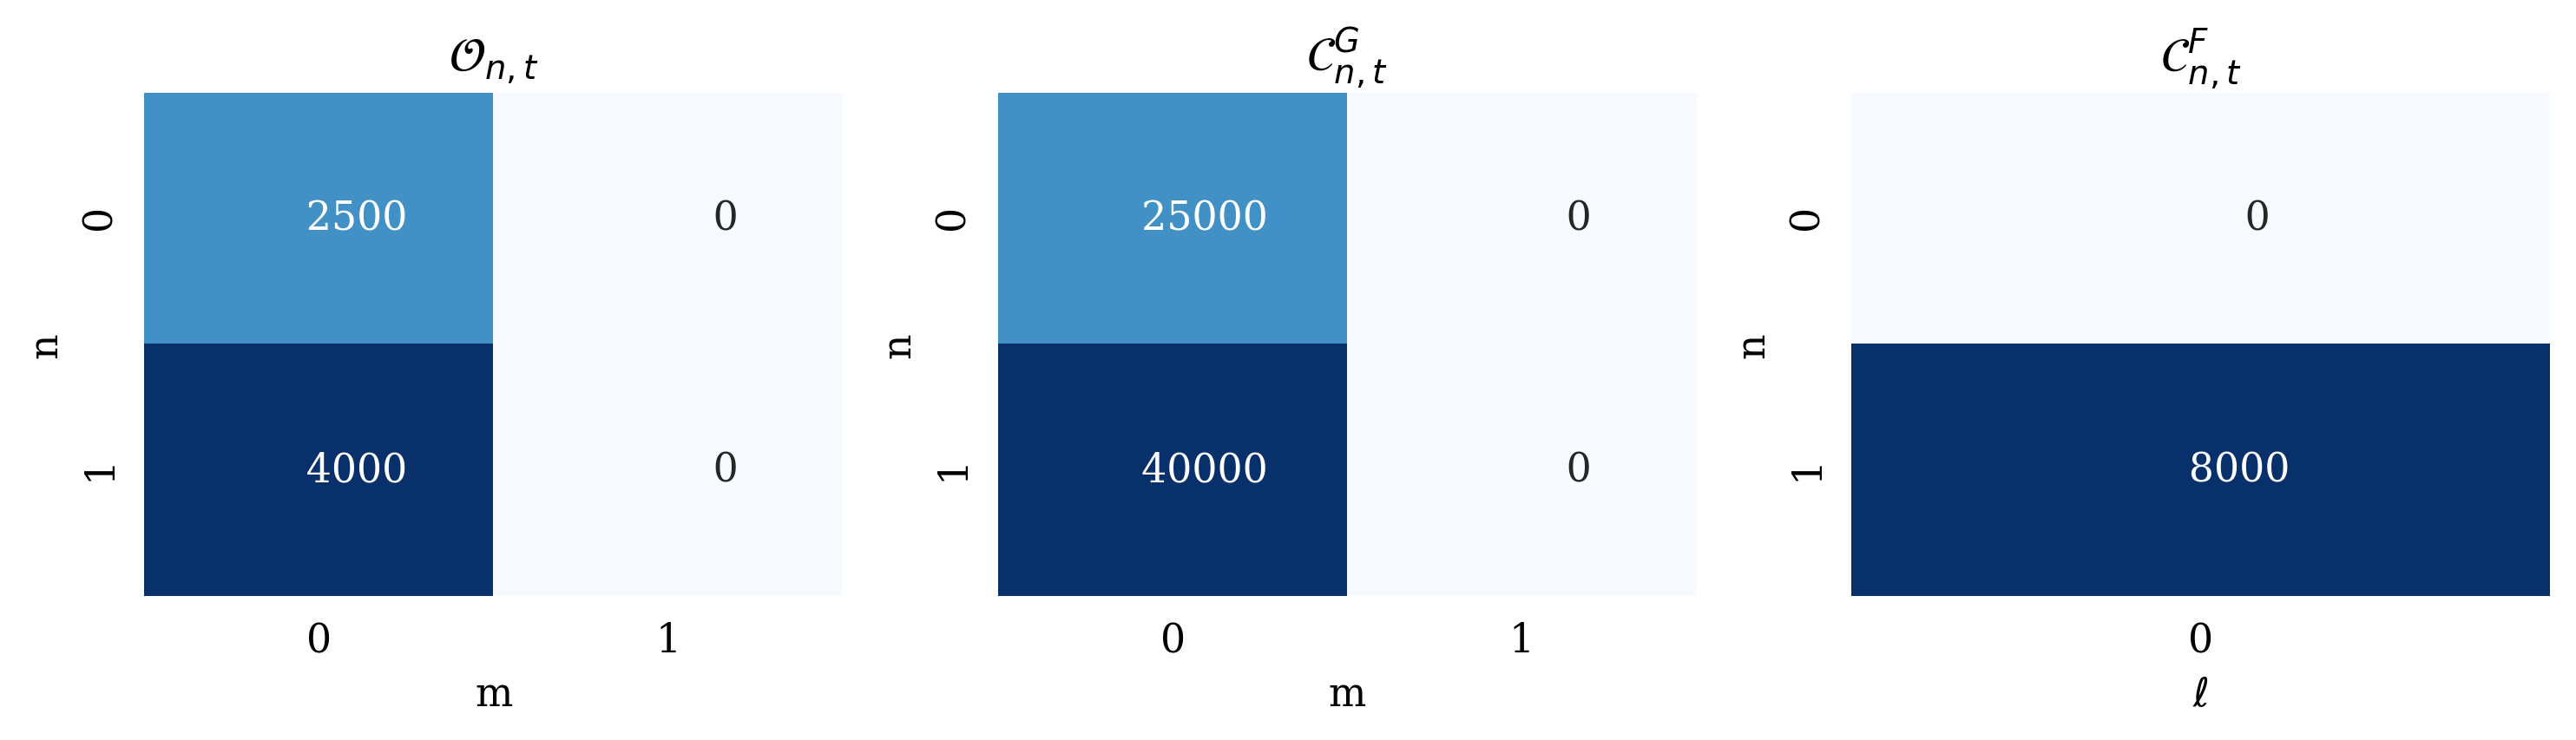
\includegraphics[width=\linewidth]{example_payoff.png}
\caption{Full P2P cost allocation for the example setup shown in \cref{fig:example_network}. The payments are derived on the basis of \cref{eq:allocate_opexGeneration_detailed,eq:allocate_capexGeneration_detailed,eq:allocate_capexFlow_detailed}. Consumers at bus $n$ have to pay each generator proportional to their consumption. As we only consider one time step the proportionality applies for OPEX $\mathcal{O}_n$ and CAPEX $\mathcal{C}_n$. As bus~1 induces a relieving flow an line~1 and therefore ``prevents`` further tranmission expansion, it is rewarded proportional to the relief.}
\label{fig:example_payoff}
\end{figure}
% 
% 
\subsubsection*{Allocating Gross Power using EBE (\ref{gross}\ref{ebe}) }

\Cref{fig:example_allocation} shows the allocated transactions on basis of equvalently traded gross power (type \ref{gross}\ref{ebe}) for both buses 1~\&~2 separately. The resulting P2P payments are given in \cref{fig:example_payoff}.
The upper graph \cref{fig:example_allocation_bus1} shows that $A_{1,1}=40$~MW at bus~1 are self-sustained. Consumers at bus~1 consequently pay 2k~\euro~OPEX and 22k~\euro~CAPEX to the generator at bus~1. The remaining 20~MW come from bus~2 and induce a subflow on line 1 of $A_{2 \rightarrow 1, 1} = -20$. As this flow is in contrary direction to the total flow, it is relieving the transmission system. This translates to a congestion reward for consumers at bus~1 of $c_{\ell=1} A_{2 \rightarrow 1, 1}$~=~2k~\euro\, which is exactly the cost that had to be spent on the transmission system if bus~1 didn't induce a relieving flow, see again \cref{fig:example_payoff}. 



The lower graph \cref{fig:example_allocation_bus2} illustrates the impact of consumption at bus~2. As $d_2$ is higher than $d_1$ the retrievements from both generators are proportionately increased as well as the OPEX and CAPEX allocations to the generators. But instead of a relieving flow, consumers at bus~2 drive the burdening flow in direction of congestion. Hence the payoff to the transmission system is positive and much higher than for bus~1.

The sum of all rows in the payoff matrix in \cref{fig:example_payoff} yields the revenues of the assets $m, \ell$. These values match their overall spendings, \textit{e.g.} the total revenue of the transmission line is 4k~\euro\, which equals the cost for investments $c_{1}\,F_{1}$. The sum of all columns yields the total payment of consumers at bus $n$. For example the sum of payments of consumers at bus~1 is 36k~\euro. This is exactly the electricity price of 600~\euro/MW times the consumption of 60~MW, $\lambda_1 d_1$. \\

The fact that OPEX and CAPEX allocations are proportional to the total consumption at a bus results from optimizing one time step only. In larger optimization problems with multiple time steps the CAPEX allocation takes effect only for time steps in which capacity contraints limit the operation of assets, \ie one or more of  \cref{eq:upper_generation_capacity_constraint,eq:lower_flow_capacity_constraint,eq:upper_flow_capacity_constraint} is binding.  

\subsubsection*{Allocating Net Power using EBE (\ref{net}\ref{ebe}) }




\section{Application Case}


\clearpage
\appendix

\section{Appendix}
\subsection{LMP from Optimization}
The nodal balance constraint ensures that the amount of power that flows into a bus equals the power that flows out of a bus, thus reflects the Kirchhoff Current Law (KCL)
\begin{align}
    \sum_l \incidence \, \flow  - \nodalgeneration + \nodaldemand &= 0 \resultsin{\lmp} \Forall{n,t}
    \label[constraint]{eq:nodal_balance_lin}
\end{align}
Its shadow price mirrors the Locational Marginal Prizes (LMP) $\lmp$ per bus and time step. In a power market this is the \euro/\megawatthour-price which a consumer has to pay. Note that the flow $\flow$ in \cref{eq:nodal_balance_lin} is a passive variable only, given by \cref{eq:flow_from_ptdf}.\\


\subsection{Proof Generation Capacity Payback}

As stated in \cite{brown_decreasing_2020} the capical cost of a generator $s$ is equal to the shadowprice $\muuppergeneration$ times the upper availibility $\generationpotential$ of all time steps 
\begin{align}
 \capexGeneration  = \sum_t \muuppergeneration \, \generationpotential 
 \label{eq:capital_price_generation_sum}
\end{align}
\Cref{eq:upper_generation_capacity_constraint,eq:lower_generation_capacity_constraint} which yield the KKT variables $\muuppergeneration$ and $\mulowergeneration$ imply the complementary slackness,
\begin{align}
\muuppergeneration \left( \generation - \generationpotential \, \capacityGeneration \right)  &= 0  \Forall{n,s,t} 
\label{eq:complementary_slackness_upper_generation} \\
\mulowergeneration  \, \generation &= 0 \Forall{n,s,t}
\label{eq:complementary_slackness_lower_generation} 
\end{align}
Multiplying both sides of \cref{eq:complementary_slackness_upper_generation} with $\capacityGeneration$ and using \cref{eq:capital_price_generation_sum} leads to 
\begin{align}
 \capexGeneration \, \capacityGeneration  = \sum_t \muuppergeneration \, \generation 
 \label{eq:capital_price_generation_sum}
\end{align}

\subsection{Proof Flow Capacity Payback}

The yielding KKT variables $\muupperflow$ and $\mulowerflow$ are only non-zero if $\flow$ is limited by the trasmission capacity in positive or negative direction, i.e. \cref{eq:upper_flow_capacity_constraint} or \cref{eq:lower_flow_capacity_constraint} are binding. The complementary slackness 
\begin{align}
\muupperflow \left( \flow - \capacityFlow \right)  &= 0 \Forall{\ell,t}
\label{eq:complementary_slackness_upper_flow} \\
\mulowerflow \left( \flow - \capacityFlow \right) &=  0 \Forall{\ell,t}
\label{eq:complementary_slackness_lower_flow} 
\end{align}
set the respective KKT for flows staying below the thermal limit to zero. 





\subsection{Full Lagrangian}
\label{sec:full_lagrangian}
\begin{align}
\notag
& \lagrangian\left(\generation, \flow, \capacityGeneration, \capacityFlow, \boldsymbol{\lambda}, \boldsymbol{\mu} \right)   =   \\  
\notag
& \;\;\; \sum_{n,s} \capexGeneration \capacityGeneration + \sum_{n, s, t} \opexGeneration \generation + \sum_{\ell} \capexFlow \, \capacityFlow  \\
\notag
&+ \sum_{n,t} \lmp \left(\sum_\ell \incidence \, \flow  - \sum_s \generation + \sum_a \demand  \right)  \\ 
\notag
&+ \sum_{\ell,c,t} \cycleprice \, \cycle \, \impedance \, \flow  \\
\notag
&+ \sum_{n,s,t} \muuppergeneration \left( \generation - \generationpotential \capacityGeneration \right)  - \sum_{n,s,t} \mulowergeneration \generation  \\
&+ \sum_{\ell,t} \muupperflow \left( \flow - \capacityFlow \right) - \sum_{\ell,t} \mulowerflow \left( \flow + \capacityFlow \right)     
\label{eq:full_lagrangian}
\end{align}
% 
where $\boldsymbol{\lambda} = \left\lbrace \lmp, \cycleprice \right\rbrace $ and $\boldsymbol{\mu} = \left\lbrace \muuppergeneration, \mulowergeneration, \muupperflow, \mulowerflow \right\rbrace $ denote the set of related KKT variables. The global maximum of the Lagrangian requires stationarity with respect to all variables. The stationarity of the generation capacity variable leads to 
\begin{align}
\pdv{\lagrangian}{\capacityGeneration}  = 0 \,\, \rightarrow \,\, 
\capexGeneration =  \sum_t \muuppergeneration \, \generationpotential  \Forall{n,s}
\label{eq:capexGeneration_duality}
\end{align}

the stationarity of the transmission capacity to
\begin{align}
\pdv{\lagrangian}{\capacityFlow} = 0 \,\, \rightarrow \,\, 
\capexFlow =  \sum_t \left( \muupperflow - \mulowerflow \right) \Forall{\ell}
\label{eq:capexFlow_duality}
\end{align}


and the stationarity of the generation to 
\begin{align}
\pdv{\lagrangian}{\generation} &= 0 \,\, \rightarrow \,\,  
\opexGeneration =  \lmp - \muuppergeneration + \mulowergeneration \Forall{n,s} \label{eq:opex_duality}
\end{align}

\subsection{CO$_2$ constraint}

Imposing an additional CO$_2$ constraint limiting the total emission to K,  
\begin{align}
\sum_{n,s,t} \emission \, \generation \le \text{K} \resultsin{\emissionPrice} 
\label[constraint]{eq:co2_constraint}
\end{align}
with $\emission$ being the emission factor in tonne-CO$_2$ per \megawatthour, returns an effective CO$_2$ price $\emissionPrice$ in \euro/tonne-CO$_2$. 
% The CO$_2$ price shifts the right hand side of the non-profit relation for generators \cref{eq:non_profit_generator} to
% 
% \begin{align}
% \capexGeneration \, \capacityGeneration + \sum_{t} \opexGeneration \, \generation &= \sum_{t} \left( \lmp - \emission \, \emissionPrice \right)  \, \generation \Forall{n,s} 
% \label{eq:non_profit_generator_emission}
% \end{align}
% This shows nicely the duality for exchanging the CO$_2$ \cref{eq:co2_constraint} for a shifted OPEX which includes the CO$_2$ costs
As shown in ... the constraint can be translated in a dual price which shift the operational price per generator
\begin{align}
\opexGeneration \rightarrow \opexGeneration + \emission \, \emissionPrice \label[relation]{eq:shift_opex_by_emission_cost}
\end{align}


\subsection{Power Transfer Distribition Factors and Flow Allocation}
\label{sec:ptdf_and_flow_allocation}


In linear power flow models, the Power Transfer Distribition Factors (PTDF) $\ptdf$ determine the changes in the flow on line $\ell$ for one unit (typically one MW) of net power production at bus $n$. Thus for a given production $\generation$ and demand $\demand$, they directly link to the the resulting flow on each line, 
\begin{align}
\flow  =   \sum_n \ptdf  \left( \nodalgeneration- \nodaldemand \right)    
\label{eq:flow_from_ptdf}
\end{align}
where $\nodalgeneration = \sum_s \generation$ and $\nodaldemand = \sum_a \demand$ combine all generators $s$ and all comsumers $a$ attached to $n$.
The PTDF have a degree of freedom: The slack $\slack$ denotes the contribution of bus $n$ to balancing out total power excess or deficit in the system. It can be dedicated to one bus, a sinlge ``slackbus``, or to several or all buses. The choice of slack modifies the PTDF according to 
\begin{align}
\ptdf\left( \slack[m]\right)  = \ptdfEqual - \sum_m \ptdfEqual[m]  \, \slack[m]
\label{eq:ptdf_slacked}
\end{align}
where $\ptdfEqual$ denote the PTDF with equally distributed slack.
When bus $n$ injects excess power, it has to flow to the slack; when bus $n$ extract deficit power, it has to come from the slack. Summing over all ingoing and outgoing flow changes resulting from a positive injection at $n$ yields again the slack 
\begin{align}
\sum_\ell \incidence[m] \, \ptdf =  \delta_{m,n} - \slack[m] 
\label{eq:slack}
\end{align}
Note that $\delta_{m,n}$ on the right hand side represents the positive injection at $n$.
% As shown above, the choice of slack $\slack[m]$ decides on the generators and lines to which power imbalances are distributed to. 
Established flow allocation schemes [cite] haved used this degree of freedom in order to allocate power flows and exchanges to market participants. Under the assumption that consumers account for all power flows in the grid, the slack is set to $\slack^*$ such that 
\begin{align}
\flow  = - \sum_n \ptdf\left( \slackk[m]\right) \, \nodaldemand  
\label{eq:flow_from_demand}
\end{align}
With such a choice the flow can be reproduced from the demand-side of the system only. Now each term in the sum on the right hand side stands for the individual contribution of consumers at node $n$ to the network flow $\flow$. In other words, each nodal demand $\nodaldemand$ induces a subflow originating from the slack $\slackk$ which all together add up to $\flow$. These subflows, in turn, can be further broken down to contributions for each bus $m$ in the slack, such that we get the subflow of individual $m \rightarrow n$ relations, that is 
\begin{align}
\allocateTransaction = \left(  \ptdfEqual[m] - \ptdfEqual \right) \slackk[m] \, \nodaldemand
\label{eq:allocate_transaction}
\end{align}
% 
It indicates the flow on line $\ell$ coming from generators at $m$ and supplying the demand $\nodaldemand$. When summing over all sources $m$ it yields the total subflow induced by $\nodaldemand$, the same term as in the sum on the right hand side in \cref{eq:flow_from_demand}; 
% \begin{align}
% \sum_m \allocateTransaction = -\ptdf\left(\slackk[m] \right) \,  \nodaldemand
% \end{align}
when summing over all sources and sinks, it yields again the power flow, thus
\begin{align}
\flow = \sum_{m,n} \allocateTransaction
\label{eq:transaction_sum}
\end{align}
% 
As mentioned before, the consumed power $\nodaldemand$ has to come from the slack $\slackk[m]$. As proofen in \cref{sec:proof_allocate_peer}, for each P2P relation $m \rightarrow n$, the ``traded`` power $\allocatePeer$  amounts to
\begin{align}
\allocatePeer &= \slackk[m] \, \nodaldemand 
\label{eq:allocate_peer}
\end{align}
% 
Finally, when summing over all sinks the P2P trades yield the nodal generation (see \cref{sec:proof_sum_n_allocate_peer}) 
\begin{align}
\sum_n \allocatePeer = \nodalgeneration[m]
\label{eq:sum_n_allocate_peer}
\end{align}
and summing over all sources yields the nodal demand 
\begin{align}
\sum_m \allocatePeer = \nodaldemand
\label{eq:sum_m_allocate_peer}
\end{align}
which follows from the fact that $\sum_n \slackk = 1$.
Both allocation quantities $\allocatePeer$ and $\allocateTransaction$ can be broken down to generators $s$ or consumers $a$ by multiplying with the nodal production share $\generationshare = \generation/\sum_s \generation$ and the nodal comsumer share $\demandshare = \demand/\sum_a \demand$ respectively. \\

The solution to $\slackk$ follows from combining \cref{eq:allocate_peer,eq:sum_n_allocate_peer}, which sets it to the share of the total production $\slackk = c \, \nodalgeneration$ with $c$ being defined as $c = 1/\sum_n \nodalgeneration$. That leads to the demand $\demand$ of every single consumers $a$ being supplied by all generators $s$ in the network proportional to their gross production $\generation$. 


\subsection{\texorpdfstring{Proof \Cref{eq:allocate_peer}}{First Proof}}
\label{sec:proof_allocate_peer}

\Cref{eq:allocate_peer} follows from summing $\allocateTransaction$ over all incoming flows to $n$ and taking into account the power that $n$ provides by itsself, $\slackk \, \nodaldemand$, which leads us to
\begin{align*}
\allocatePeer &= \slackk \, \nodaldemand - \sum_{\ell} \incidence \, \allocateTransaction \\
&= \slackk \, \nodaldemand - \sum_\ell \incidence \left(  \ptdfEqual[m] - \ptdfEqual \right) \slackk[m] \, \nodaldemand  \\
&= \slackk \, \nodaldemand - \left(  \delta_{n,m} - \dfrac{1}{N} - \delta_{n,n} + \dfrac{1}{N} \right) \slackk[m] \, \nodaldemand  \\
&= \slackk \, \nodaldemand - \left(  \delta_{n,m} - 1 \right) \slackk[m] \, \nodaldemand  \\
&= \slackk[m] \, \nodaldemand 
\end{align*}
where we used \cref{eq:slack} and the fact that the equally distributed slack amounts to $1/N$ for all N nodes in the network. 



\subsection{\texorpdfstring{Proof of \Cref{eq:sum_n_allocate_peer}}{Second proof}}
\label{sec:proof_sum_n_allocate_peer}
The relation follows from multiplying \cref{eq:flow_from_demand} with $\sum_m \incidence[m]$, and solving for $\allocatePeer$
\begin{align*}
\sum_m \incidence[m] \, \flow &= - \sum_{m,n} \incidence[m] \, \ptdf \, \nodaldemand \\
\nodalgeneration[m] - \nodaldemand[m] &= - \delta_{m,n} \, \nodaldemand + \slackk[m] \, \nodaldemand    \\
\allocatePeer &= \nodalgeneration[m] - \nodaldemand[m] + \delta_{m,n} \nodaldemand \\
\sum_n \allocatePeer &= \nodalgeneration[m]
\end{align*}

\subsection{Allocating Gross Injections with EBE}
\label{sec:gross_ebe}
Allocating gross injections using the Equivalent Bilateral Exchanges Principal is simplistic and straightforward scheme. Accordingly each generator supplies each bus proportional to its power demand. The allocation is given by 
\begin{align}
 \allocatePeer = \dfrac{\generation}{\sum_s \generation} \demand 
\end{align}


\subsection{Allocating Net Injections with EBE}
\label{sec:net_ebe}

Allocating net power injections using the EBE methods leads to the same result as the Marginal Participation (MP) \cite{rudnick_marginal_1995}  algorithm when allocating to consumers only, see \cite{hofmann_flow_2020-1} for further insight. We calculate it by setting 
\begin{align}
\allocatePeer[m \rightarrow n] &=  \delta_{m,n}\,\selfconsumption[m] + \gamma_t \, \netconsumption  \, \netproduction[m]
\label{eq:mp_slack}
\end{align}
where 
\begin{itemize}
%  \item $\injection = \left( \nodalgeneration - \nodaldemand \right) $ denotes the nodal injection
\item $\netproduction = \text{min}\left( \nodalgeneration - \nodaldemand , 0 \right) $ denotes the nodal net production 
\item $\netconsumption = \text{min}\left( \nodaldemand  - \nodalgeneration, 0 \right)$ denotes the nodal net consumption
\item $\selfconsumption = \text{min}\left( \netproduction, \netconsumption \right)$ the denotes  nodal self-consumption. That is the power generated and at the same time consumed at node $n$ and 
\item $\gamma_t = \left( \sum_n \netproduction\right) ^{-1} = \left( \sum_n \netconsumption\right) ^{-1}$ is the inverse of the total injected/extracted power at time $t$.
\end{itemize}

The allocation $\allocatePeer$ from generator $s$ to $n$, is given by multiplying $\allocatePeer[m \rightarrow n]$ with the nodal share $\generation / \nodalgeneration$.


\subsection{Allocating Net Power using AP}
\label{sec:net_ap}

\newcommand{\incidenceM}{K}
\newcommand{\flowM}{f}
\newcommand{\injectionM}{p}
\newcommand{\slackM}{k}
\newcommand{\DirectedIncidence}{\mathcal{K}}
\newcommand{\InverseAPInjection}{\mathcal{J}}
\newcommand\diag[1]{\operatorname{diag}\left(#1\right)}


Allocating net injections using the AP method is derived from \cite{achayuthakan_electricity_2010-1}. In a lossless network the downstream and upstream formulations result in the same P2P allocation which is why we restrict ourselves to the downstream formulation only. In a first step we define a time-dependent auxiliary matrix $\InverseAPInjection_t$ which is the inverse of the $N\times N$ with directed power flow $m \rightarrow n$ at entry $(m, n)$ for $m \ne n$ and the total flow passing node $m$ at entry $\left( m, m\right)$ at time step $t$. Mathematically this translates to


\begin{align}
\InverseAPInjection_t = \left( \diag{\injectionM^+} + \DirectedIncidence^- \diag{\flowM} \, \incidenceM \right)_t^{-1} 
\end{align}
where $\DirectedIncidence^-$ is the negative part of the directed Incidence matrix $\DirectedIncidence_{n,\ell} = \text{sign}\left( \flow \right)  \incidence$. Then the distributed slack for time step $t$ is given by
\begin{align}
\allocatePeer[m \rightarrow n] = \InverseAPInjection_{m,n,t} \, \netproduction[m] \, \netconsumption
\end{align}

\subsection{Allocating Gross Power using AP}
\label{sec:gross_ap}

We use the same allocation as in \cref{sec:net_ap} but replace the net nodal production $\netproduction$ by the gross nodal production $\nodalgeneration$ which leads to  
\begin{align}
\InverseAPInjection_t = \left( \diag{g} + \DirectedIncidence^- \diag{\flowM} \, \incidenceM \right)_t^{-1} 
\end{align}
The distributed slack is for time step $t$ is then given by
\begin{align}
\allocatePeer[s \rightarrow m] = \InverseAPInjection_{m,n} \, \generation \, \demand
\end{align}



\clearpage
\printbibliography




\end{document}
